\documentclass[12pt]{article}
\usepackage[margin=1in]{geometry}

\usepackage{libertine}
\usepackage{parskip}
\usepackage{graphicx}
\graphicspath{ {./images/} }

\usepackage{amsthm,amsmath,amssymb}
\usepackage{tikz}
\usetikzlibrary{arrows,automata,shapes.geometric}

\usepackage{pgfplots}
\pgfplotsset{compat=1.18}

\pagestyle{plain}
\thispagestyle{empty}

\definecolor{carnellian}{RGB}{190,20,20}

\theoremstyle{definition}
\newtheorem{problem}{Problem}

\newcounter{subq}[problem]
\newenvironment{subproblem}
{\refstepcounter{subq} \begin{itemize} \item[(\alph{subq})]}
{\end{itemize} \medskip}

\usepackage{environ}
\NewEnviron{solution}[1][\vfill]{
    \textcolor{blue}{\BODY}
}

\newcommand{\hwnum}{1}
\newcommand{\duedate}{9/8/2024}
\renewcommand{\title}{Fields}

\begin{document}

\hspace{-10px}
\begin{tabular*}{\textwidth}{l @{\extracolsep{\fill}} r}
    \textbf{Honors Linear Algebra} 
        & \textbf{Fall 2024} \\
    \textbf{HW\hwnum: \title} &  \textbf{Due: \duedate}
\end{tabular*}

\vspace{1cm}

\begin{problem}
    Verify that the set of complex numbers described in Example 4 is a subfield of $C$. 
    
    Example 4. The set of all complex numbers of the form $x + y\sqrt{2}$, where $x$ and $y$
    are rational, is a subfield of $C$. We leave it to the reader to verify this.

    \begin{solution}
        1. (+) Commutativity:\\
        For any two elements \( a = x_1 + y_1\sqrt{2} \) and \( b = x_2 + y_2\sqrt{2} \) $\in$ \( F \):
        \[
        a + b = (x_1 + y_1\sqrt{2}) + (x_2 + y_2\sqrt{2}) = (x_1 + x_2) + (y_1 + y_2)\sqrt{2}
        \]
        Since \( x_1 + x_2 = x_2 + x_1 \) and \( y_1 + y_2 = y_2 + y_1 \) (commutativity in \( \mathbb{Q} \)), addition in \( F \) is commutative.

        2. (+) Associativity:\\
        For any three elements \( a = x_1 + y_1\sqrt{2} \), \( b = x_2 + y_2\sqrt{2} \), and \( c = x_3 + y_3\sqrt{2} \) $\in$ \( F \):
        \[
        (a + b) + c = \left( (x_1 + y_1\sqrt{2}) + (x_2 + y_2\sqrt{2}) \right) + (x_3 + y_3\sqrt{2})
        \]
        \[
        = (x_1 + x_2 + x_3) + (y_1 + y_2 + y_3)\sqrt{2}
        \]
        Similarly:
        \[
        a + (b + c) = (x_1 + (x_2 + x_3)) + (y_1 + (y_2 + y_3))\sqrt{2}
        \]
        Since addition is associative in \( \mathbb{Q} \), addition in \( F \) is also associative.
        
        3. (+) There is a unique element $0$ element $\in \mathbb{F}$:\\
        The element \( 0 + 0\sqrt{2} = 0 \) is the additive identity in \( F \), and it satisfies:
        \[
        a + 0 = (x + y\sqrt{2}) + 0 = x + y\sqrt{2}
        \]
        Thus, \( 0 \) is the unique additive identity.

        4. (+) To each $x \in \mathbb{F}$ there corresponds a unique element $(-x) \in \mathbb{F}$ such that $x + (-x) = 0$:\\
        For any element \( a = x + y\sqrt{2} \in F \), the element \( -a = -x - y\sqrt{2} \in F \) satisfies:
        \[
        a + (-a) = (x + y\sqrt{2}) + (-x - y\sqrt{2}) = (x - x) + (y - y)\sqrt{2} = 0
        \]
        Thus, \( -a \in F \) is the unique additive inverse of \( a \).

        5. ( $\cdot$ ) Multiplication is Commutative:\\
        For any two elements \( a = x_1 + y_1\sqrt{2} \) and \( b = x_2 + y_2\sqrt{2} \) $\in$ \( F \):
        \[
        a \cdot b = (x_1 + y_1\sqrt{2})(x_2 + y_2\sqrt{2}) = x_1x_2 + (x_1y_2 + y_1x_2)\sqrt{2} + 2y_1y_2
        \]
        \[
        = (x_1x_2 + 2y_1y_2) + (x_1y_2 + y_1x_2)\sqrt{2}
        \]
        Multiplication in \( \mathbb{Q} \) is commutative, so multiplication in \( F \) is also commutative.

        6. ( $\cdot$ ) Multiplication is Associative:\\
        For any three elements \( a = x_1 + y_1\sqrt{2} \), \( b = x_2 + y_2\sqrt{2} \), and \( c = x_3 + y_3\sqrt{2} \) in \( F \):
        \[
        (a \cdot b) \cdot c = \left( (x_1 + y_1\sqrt{2})(x_2 + y_2\sqrt{2}) \right) \cdot (x_3 + y_3\sqrt{2})
        \]
        The result will simplify similarly to the earlier case, and because multiplication is associative in \( \mathbb{Q} \), it is associative in \( F \).

        7. ( $\cdot$ ) There is a unique non-zero element $1 \in \mathbb{F}$ such that $x1 = x$, for every $x\in\mathbb{F}$:\\
        The element \( 1 + 0\sqrt{2} = 1 \) is the multiplicative identity in \( F \), and it satisfies:
        \[
        a \cdot 1 = (x + y\sqrt{2})(1 + 0\sqrt{2}) = x + y\sqrt{2}
        \]
        Thus, \( 1 \) is the unique multiplicative identity.

        8. ( $\cdot$ ) To each non-zero $x \in\mathbb{F}$ there corresponds a unique element $x^{-1}\in\mathbb{F}$ such that $xx^{-1} = 1$:\\
        Let \( a = x + y\sqrt{2} \in F \), where \( a \neq 0 \). To find \( a^{-1} \), multiply by the conjugate:
        \[
        a^{-1} = \frac{1}{a} = \frac{1}{x + y\sqrt{2}} \cdot \frac{x - y\sqrt{2}}{x - y\sqrt{2}} = \frac{x - y\sqrt{2}}{x^2 - 2y^2}
        \]
        Since \( x^2 - 2y^2 \neq 0 \) (because \( a \neq 0 \)) and both the numerator and denominator are in \( F \), we conclude that \( a^{-1} \in F \). Thus, every non-zero element has a unique multiplicative inverse in \( F \).

        9. ( $\cdot$, + ) Multiplication distributes over Addition:\\
        For any \( a = x_1 + y_1\sqrt{2} \), \( b = x_2 + y_2\sqrt{2} \), and \( c = x_3 + y_3\sqrt{2} \) in \( F \):
        \[
        a \cdot (b + c) = (x_1 + y_1\sqrt{2}) \cdot ((x_2 + y_2\sqrt{2}) + (x_3 + y_3\sqrt{2}))
        \]
        \[
        = (x_1 + y_1\sqrt{2}) \cdot (x_2 + x_3 + (y_2 + y_3)\sqrt{2})
        \]
        Expanding this confirms that multiplication distributes over addition, just like in \( \mathbb{Q} \).

        Conclusion: Since all the required properties hold, the set \( F = \{ x + y\sqrt{2} \mid x, y \in \mathbb{Q} \} \) satisfies the field axioms and is therefore a subfield of \( \mathbb{C} \).

    \end{solution}
\end{problem}

\begin{problem}[Problem 1 from Extra Problems]
    The smallest subfield of a field $\mathbb{F}$ is called the prime subfield of $\mathbb{F}$.

    \begin{subproblem}
        Show that the prime subfield of $\mathbb{F}$ consists of all elements which can be written as $ab^{-1}$, where $a$ and $b \neq 0$ are multiples of 1, i.e. elements of the form $n \cdot 1 = 1 + 1 + \ldots + 1$ ($n$ times).

        \begin{solution}
            Consider the set of all elements in \( \mathbb{F} \) that can be written as \( ab^{-1} \), where \( a \) and \( b \) are integer multiples of the multiplicative identity \( 1 \) in \( \mathbb{F} \). Explicitly, these elements are of the form \( n \cdot 1 \), where \( n \) is an integer, and can be expressed as sums or differences of 1 in \( \mathbb{F} \). Such elements include \( 1, -1, 0, 2, -2, \ldots \), forming a copy of the integers within \( \mathbb{F} \).

            The inverses of non-zero elements of this form, consider the element \( b = n \cdot 1 \), where \( n \neq 0 \). The inverse \( b^{-1} \) must also exist in \( \mathbb{F} \). Therefore, any element of the form \( ab^{-1} \), where \( a = m \cdot 1 \) and \( b = n \cdot 1 \), will be a rational number, i.e., an element of \( \mathbb{Q} \), the field of rational numbers.
    
            The prime subfield must be the smallest subfield of \( \mathbb{F} \) that contains \( 1 \) and is closed under addition, multiplication, and the axioms for a Field. The set of all elements of the form \( ab^{-1} \), where \( a, b \in \mathbb{Z} \) and \( b \neq 0 \), corresponds to the field of rational numbers \( \mathbb{Q} \) in characteristic 0, or the finite field \( \mathbb{Z}/\mathbb{Z}_p \) in characteristic \( p \). These are the smallest subfields that exist within \( \mathbb{F} \), thus forming the prime subfield.
    
            Therefore, the prime subfield of \( \mathbb{F} \) consists of all elements of the form \( ab^{-1} \), where \( a \) and \( b \neq 0 \) are integer multiples of 1.
        \end{solution}
    \end{subproblem}

    \begin{subproblem}
        Show that any prime subfield is isomorphic to either $\mathbb{Q}$ or $\mathbb{F}_p$.
        \begin{solution}

        Two cases arise based on the characteristic of the field \( \mathbb{F} \):

        Case 1: The characteristic of \( \mathbb{F} \) is 0.\\
        The additive structure of the prime subfield is isomorphic to the integers \( \mathbb{Z} \), and since the prime subfield must also include the multiplicative inverses of non-zero elements, we obtain the field of rational numbers \( \mathbb{Q} \). Therefore, if \( \mathbb{F} \) has characteristic 0, its prime subfield is isomorphic to \( \mathbb{Q} \).

        Case 2: The characteristic of \( \mathbb{F} \) is \( p > 0 \).\\
        \( p \cdot 1 = 0 \) for some prime \( p \). Thus, the additive structure of the prime subfield is isomorphic to \( \mathbb{Z}/\mathbb{Z}_p \), as shown in part (a). Since the prime subfield is closed under addition, multiplication, and inverses, this subfield must be isomorphic to the finite field \( \mathbb{F}_p = \mathbb{Z}/\mathbb{Z}_p \).

        Thus, any prime subfield is either isomorphic to \( \mathbb{Q} \) if the characteristic of the field is 0, or isomorphic to \( \mathbb{F}_p \) if the characteristic of the field is \( p > 0 \). These are the only possible prime subfields.
        \end{solution}
    \end{subproblem}
\end{problem}

\begin{problem}[Problem 2 from Extra Problems]
    (Fields)
    \begin{subproblem}
        Let $\mathbb{Q}[\sqrt[3]{2}]$ denote the minimal subfield of $\mathbb{C}$ which contains $\sqrt[3]{2}$. Give an explicit description of this field (as a set) and show directly that it is a field.
        \begin{solution}

            The field \( \mathbb{Q}[\sqrt[3]{2}] \) is the smallest subfield of \( \mathbb{C} \) that contains both the rationals \( \mathbb{Q} \) and the element \( \sqrt[3]{2} \). Therefore, it consists of all elements of the form:
            \[
            \mathbb{Q}[\sqrt[3]{2}] = \left\{ a + b \sqrt[3]{2} + c \sqrt[3]{4} \mid a, b, c \in \mathbb{Q} \right\}
            \]
            where \( a, b, c \) are rational numbers and \( \sqrt[3]{2} \) is a root of the polynomial \( x^3 - 2 = 0 \).

            Now, verifying that \( \mathbb{Q}[\sqrt[3]{2}] \) is a field:

            1. (+) Commutativity:\\
            For any \( f = a_1 + b_1 \sqrt[3]{2} + c_1 \sqrt[3]{4} \) and \( g = a_2 + b_2 \sqrt[3]{2} + c_2 \sqrt[3]{4} \), 
            \[
            f + g = (a_1 + a_2) + (b_1 + b_2) \sqrt[3]{2} + (c_1 + c_2) \sqrt[3]{4}
            \]
            is the same as \( g + f \), so addition is commutative.

            2. (+) Associativity:\\
            For any three elements \( f = a_1 + b_1 \sqrt[3]{2} + c_1 \sqrt[3]{4} \), \( g = a_2 + b_2 \sqrt[3]{2} + c_2 \sqrt[3]{4} \), and \( h = a_3 + b_3 \sqrt[3]{2} + c_3 \sqrt[3]{4} \), 
            \[
            (f + g) + h = f + (g + h)
            \]
            holds by the associativity of addition in \( \mathbb{Q} \).

            3. (+) There is a unique element $0$ element $\in \mathbb{F}$:\\
            The element \( 0 = 0 + 0 \sqrt[3]{2} + 0 \sqrt[3]{4} \) is the additive identity since for any element \( f = a + b \sqrt[3]{2} + c \sqrt[3]{4} \),
            \[
            f + 0 = f
            \]
            and \( 0 + f = f \).

            4. (+) To each $x \in \mathbb{F}$ there corresponds a unique element $(-x) \in \mathbb{F}$ such that $x + (-x) = 0$:\\
            For any \( f = a + b \sqrt[3]{2} + c \sqrt[3]{4} \), the additive inverse is \( -f = -a - b \sqrt[3]{2} - c \sqrt[3]{4} \), such that 
            \[
            f + (-f) = 0.
            \]

            5. ( $\cdot$ ) Multiplication is Commutative:\\
            For any \( f = a_1 + b_1 \sqrt[3]{2} + c_1 \sqrt[3]{4} \) and \( g = a_2 + b_2 \sqrt[3]{2} + c_2 \sqrt[3]{4} \),
            \[
            f \cdot g = g \cdot f
            \]
            holds by the commutativity of multiplication in \( \mathbb{Q} \).

            6. ( $\cdot$ ) Multiplication is Associative:\\
            The associativity of multiplication in \( \mathbb{Q} \) ensures that 
            \[
            (f \cdot g) \cdot h = f \cdot (g \cdot h)
            \]
            for any \( f, g, h \in \mathbb{Q}[\sqrt[3]{2}] \).

            7. ( $\cdot$ ) There is a unique non-zero element $1 \in \mathbb{F}$ such that $x1 = x$, for every $x\in\mathbb{F}$:\\
            The element \( 1 = 1 + 0 \sqrt[3]{2} + 0 \sqrt[3]{4} \) is the multiplicative identity since for any element \( f = a + b \sqrt[3]{2} + c \sqrt[3]{4} \),
            \[
            f \cdot 1 = f
            \]
            and \( 1 \cdot f = f \).

            8. ( $\cdot$ ) To each non-zero $x \in\mathbb{F}$ there corresponds a unique element $x^{-1}\in\mathbb{F}$ such that $xx^{-1} = 1$:\\
            For any non-zero element \( f = a + b \sqrt[3]{2} + c \sqrt[3]{4} \), the inverse \( f^{-1} \in \mathbb{Q}[\sqrt[3]{2}] \) exists (it can be computed by multiplying by conjugates and rationalizing the denominator, as done with similar algebraic numbers).

            9. ( $\cdot$, + ) Multiplication distributes over Addition:\\
            \[
            f \cdot (g + h) = f \cdot g + f \cdot h
            \]
            holds by distributivity in \( \mathbb{Q} \).

            Since \( \mathbb{Q}[\sqrt[3]{2}] \) satisfies all the field axioms, it is a field.
        \end{solution}
    \end{subproblem}

    \begin{subproblem}
        Let $\mathbb{Q}[\sqrt{2}, \sqrt{3}]$ denote the minimal subfield of $\mathbb{C}$ which contains $\sqrt{2}$ and $\sqrt{3}$. Give an explicit description of this field (as a set) and show directly that it is a field.
        \begin{solution}
            
        1. (+) Commutativity:\\ 
        Let \( f = a_1 + b_1 \sqrt{2} + c_1 \sqrt{3} + d_1 \sqrt{6} \) and \( g = a_2 + b_2 \sqrt{2} + c_2 \sqrt{3} + d_2 \sqrt{6} \). Then:
        \[
        f + g = (a_1 + a_2) + (b_1 + b_2) \sqrt{2} + (c_1 + c_2) \sqrt{3} + (d_1 + d_2) \sqrt{6}.
        \]
        Since addition in \( \mathbb{Q} \) is commutative, we have:
        \[
        f + g = g + f.
        \]
        Hence, addition is commutative.

        2. (+) Associativity:\\ 
        Let \( f = a_1 + b_1 \sqrt{2} + c_1 \sqrt{3} + d_1 \sqrt{6} \), \( g = a_2 + b_2 \sqrt{2} + c_2 \sqrt{3} + d_2 \sqrt{6} \), and \( h = a_3 + b_3 \sqrt{2} + c_3 \sqrt{3} + d_3 \sqrt{6} \). Then:
        \[
        (f + g) + h = \left( (a_1 + a_2) + (b_1 + b_2) \sqrt{2} + (c_1 + c_2) \sqrt{3} + (d_1 + d_2) \sqrt{6} \right) + (a_3 + b_3 \sqrt{2} + c_3 \sqrt{3} + d_3 \sqrt{6})
        \]
        Simplifying:
        \[
        (f + g) + h = (a_1 + a_2 + a_3) + (b_1 + b_2 + b_3) \sqrt{2} + (c_1 + c_2 + c_3) \sqrt{3} + (d_1 + d_2 + d_3) \sqrt{6}.
        \]
        Similarly:
        \[
        f + (g + h) = a_1 + (a_2 + a_3) + b_1 \sqrt{2} + (b_2 + b_3) \sqrt{2} + c_1 \sqrt{3} + (c_2 + c_3) \sqrt{3} + d_1 \sqrt{6} + (d_2 + d_3) \sqrt{6}.
        \]
        Therefore, \( (f + g) + h = f + (g + h) \), so addition is associative.

        3. (+) There is a unique element $0$ element $\in \mathbb{F}$:\\
        The element \( 0 = 0 + 0 \sqrt{2} + 0 \sqrt{3} + 0 \sqrt{6} \) is the additive identity. For any element \( f = a + b \sqrt{2} + c \sqrt{3} + d \sqrt{6} \), we have:
        \[
        f + 0 = a + b \sqrt{2} + c \sqrt{3} + d \sqrt{6}.
        \]
        Thus, \( 0 \) is the additive identity.

        4. (+) To each $x \in \mathbb{F}$ there corresponds a unique element $(-x) \in \mathbb{F}$ such that $x + (-x) = 0$:\\
        For any element \( f = a + b \sqrt{2} + c \sqrt{3} + d \sqrt{6} \), the additive inverse is \( -f = -a - b \sqrt{2} - c \sqrt{3} - d \sqrt{6} \). We check:
        \[
        f + (-f) = (a + b \sqrt{2} + c \sqrt{3} + d \sqrt{6}) + (-a - b \sqrt{2} - c \sqrt{3} - d \sqrt{6}) = 0.
        \]
        Hence, every element has an additive inverse.

        5. ( $\cdot$ ) Multiplication is Commutative:\\
        Let \( f = a_1 + b_1 \sqrt{2} + c_1 \sqrt{3} + d_1 \sqrt{6} \) and \( g = a_2 + b_2 \sqrt{2} + c_2 \sqrt{3} + d_2 \sqrt{6} \). Then the product \( f \cdot g \) is:
        \[
        f \cdot g = (a_1 + b_1 \sqrt{2} + c_1 \sqrt{3} + d_1 \sqrt{6}) \cdot (a_2 + b_2 \sqrt{2} + c_2 \sqrt{3} + d_2 \sqrt{6}).
        \]
        Expanding this expression:
        \[
        f \cdot g = a_1 a_2 + b_1 b_2 \cdot 2 + c_1 c_2 \cdot 3 + d_1 d_2 \cdot 6 + \text{other terms involving cross-products}.
        \]
        Since multiplication in \( \mathbb{Q} \) is commutative, we conclude that \( f \cdot g = g \cdot f \).

        6. ( $\cdot$ ) Multiplication is Associative:\\
        For any three elements \( f, g, h \in \mathbb{Q}[\sqrt{2}, \sqrt{3}] \), the product \( f \cdot (g \cdot h) = (f \cdot g) \cdot h \) follows by the associativity of multiplication in \( \mathbb{Q} \) and the rules of multiplying algebraic terms.

        7. ( $\cdot$ ) There is a unique non-zero element $1 \in \mathbb{F}$ such that $x1 = x$, for every $x\in\mathbb{F}$:\\
        The element \( 1 = 1 + 0 \sqrt{2} + 0 \sqrt{3} + 0 \sqrt{6} \) is the multiplicative identity. For any \( f = a + b \sqrt{2} + c \sqrt{3} + d \sqrt{6} \), we have:
        \[
        f \cdot 1 = a + b \sqrt{2} + c \sqrt{3} + d \sqrt{6}.
        \]
        Therefore, \( 1 \) is the multiplicative identity.

        8. ( $\cdot$ ) To each non-zero $x \in\mathbb{F}$ there corresponds a unique element $x^{-1}\in\mathbb{F}$ such that $xx^{-1} = 1$:\\
        For any non-zero element \( f = a + b \sqrt{2} + c \sqrt{3} + d \sqrt{6} \), there exists an inverse \( f^{-1} \in \mathbb{Q}[\sqrt{2}, \sqrt{3}] \). For example, for \( \sqrt{2} \), the inverse is \( \frac{1}{\sqrt{2}} = \frac{\sqrt{2}}{2} \), and similar procedures can be applied to compute the inverses of other elements in \( \mathbb{Q}[\sqrt{2}, \sqrt{3}] \).

        9. ( $\cdot$, + ) Multiplication distributes over Addition:\\
        For any \( f, g, h \in \mathbb{Q}[\sqrt{2}, \sqrt{3}] \), we verify that multiplication distributes over addition:
        \[
        f \cdot (g + h) = f \cdot g + f \cdot h.
        \]
        This holds by expanding both sides and applying the distributive property in \( \mathbb{Q} \).

        Hence, \( \mathbb{Q}[\sqrt{2}, \sqrt{3}] \) satisfies all the field axioms and is indeed a field.
    
        \end{solution}
    \end{subproblem}
\end{problem}

\begin{problem}[Problem 3 from Extra Problems]

    Show that there exist fields of 9 and 25 elements. Can you show that
    any two fields with 9 elements are isomorphic? (Hint: Use an element which
    behaves like $\sqrt{2}$).

    \begin{solution}
        Showing existence of a field with 9 elements:\\
        The number of elements in a finite field is always a power of a prime. To find a field with 9 elements, we note that \(9 = 3^2\). Hence, we need to construct a finite field \(\mathbb{F}_{3^2}\), a field with \(3^2 = 9\) elements.

        One way to construct a finite field of size \(p^n\) is to start with the prime field \(\mathbb{F}_p\), where \(p\) is a prime, and then find an irreducible polynomial of degree \(n\) over \(\mathbb{F}_p\).

        The elements of \(\mathbb{F}_3\) are \(\{ 0, 1, 2 \}\), and we need to find a polynomial of degree 2 over \(\mathbb{F}_3\). One such polynomial is \(f(x) = x^2 + 1\), which is irreducible over \(\mathbb{F}_3\) because it has no roots in \(\mathbb{F}_3\). That is, none of the elements \(0, 1, 2\) satisfy \(x^2 + 1 = 0\).

        Therefore, we can construct the field \(\mathbb{F}_{9}\) as \(\mathbb{F}_3[x]/(x^2 + 1)\). The elements of this field are of the form \(a + bx\), where \(a, b \in \mathbb{F}_3\), and \(x^2 = -1\) (which is equivalent to \(x^2 = 2\) in \(\mathbb{F}_3\)).

        Thus, the elements of \(\mathbb{F}_9\) are \(\{ 0, 1, 2, x, x+1, x+2, 2x, 2x+1, 2x+2 \}\).

        Now showing existence of a field with 25 elements:\\
        Similarly, 25 is \(5^2\), so we are looking for a finite field with 25 elements, \(\mathbb{F}_{25} = \mathbb{F}_{5^2}\). The elements of the prime field \(\mathbb{F}_5\) are \(\{ 0, 1, 2, 3, 4 \}\), and we need to find an irreducible polynomial of degree 2 over \(\mathbb{F}_5\).

        One such polynomial is \(f(x) = x^2 + 2\), which is irreducible over \(\mathbb{F}_5\) because it has no roots in \(\mathbb{F}_5\). Thus, we can construct \(\mathbb{F}_{25}\) as \(\mathbb{F}_5[x]/(x^2 + 2)\).

        Any two fields with 9 elements are isomorphic:\\
        It is true that any two finite fields of the same size are isomorphic. 
        Consider the field \(\mathbb{F}_9 = \mathbb{F}_3[x]/(x^2 + 1)\). The element \(x\) in this field satisfies \(x^2 = -1\), which corresponds to \(x^2 = 2\) in \(\mathbb{F}_3\). This element \(x\) behaves like \(\sqrt{2}\) in the sense that its square gives 2. Therefore, any other field of 9 elements will have an element that satisfies the same relation, and this gives a way to construct an isomorphism between any two fields of 9 elements by mapping the corresponding elements that satisfy \(x^2 = 2\).

        Thus, any two fields with 9 elements are isomorphic.
    \end{solution}

\end{problem}

\begin{problem}
    Prove that the interchange of two rows of a matrix can be accomplished by a finite sequence of elementary row operations of the other two types.
    
    \begin{solution}
        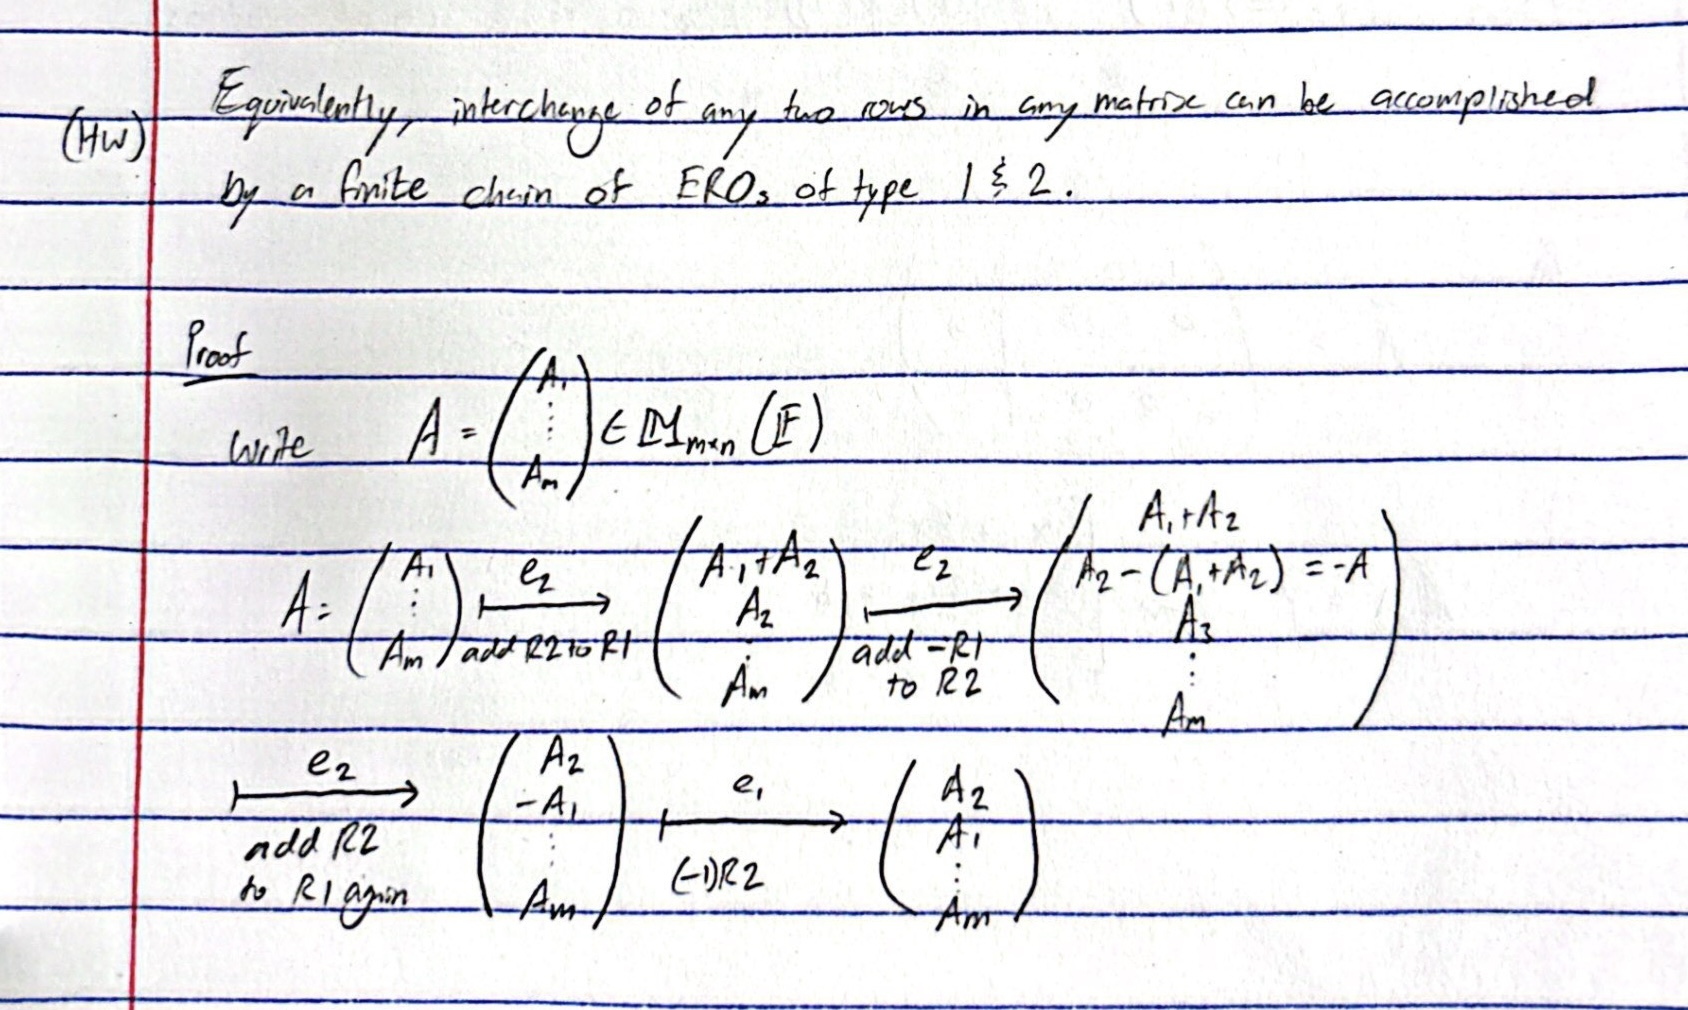
\includegraphics[scale=0.25]{p7.jpg}
    \end{solution}
\end{problem}

\clearpage

\begin{problem}
    Let
    \[
    \begin{bmatrix}
        3 & -6 & 2 & -1\\
        -2 & 4 & 1 & 3\\
        0 & 0 & 1 & 1\\
        1 & -2 & 1 & 0
    \end{bmatrix}
    \]
    For which $(y_1, y_2, y_3, y_4)$ does the system of equations $AX = Y$ have a solution?

    \begin{solution}
        To find the values of \( (y_1, y_2, y_3, y_4) \) for which the system \( AX = Y \) has a solution, we need to check the consistency of the augmented matrix \( [A|Y] \).
        \[
        \left[ \begin{array}{cccc|c}
        3 & -6 & 2 & -1 & y_1 \\
        -2 & 4 & 1 & 3 & y_2 \\
        0 & 0 & 1 & 1 & y_3 \\
        1 & -2 & 1 & 0 & y_4
        \end{array} \right]
        \]
        \[
        \left[ \begin{array}{cccc|c}
        1 & -2 & \frac{2}{3} & -\frac{1}{3} & \frac{y_1}{3} \\
        -2 & 4 & 1 & 3 & y_2 \\
        0 & 0 & 1 & 1 & y_3 \\
        1 & -2 & 1 & 0 & y_4
        \end{array} \right]
        \]
        \[
        \left[ \begin{array}{cccc|c}
        1 & -2 & \frac{2}{3} & -\frac{1}{3} & \frac{y_1}{3} \\
        0 & 0 & \frac{7}{3} & \frac{7}{3} & \frac{3y_1 + y_2}{3} \\
        0 & 0 & 1 & 1 & y_3 \\
        0 & 0 & \frac{1}{3} & \frac{1}{3} & \frac{y_4 - y_1}{3}
        \end{array} \right]
        \]
        Therefore, the system has a solution if and only if the right-hand side \( (y_1, y_2, y_3, y_4) \) satisfies the consistency conditions that come from the row reduction. This will result in specific relations between \( y_1, y_2, y_3, y_4 \).
    \end{solution}
\end{problem}

\begin{problem}
    Let
    \[
    C =
    \begin{bmatrix}
        C_{11} & C_{12}\\
        C_{21} & c_{22} 
    \end{bmatrix}
    \]
    be a 2 $\times$ 2 matrix. We inquire when it is possible to find 2 $\times$ 2 matrices $A$ and $B$ such that $C = AB - BA$. Prove that such matrices can be found if and only if $C_{11} + C_{22} = 0$.
    
    \begin{solution}


        Let \( A = \begin{bmatrix} a_{11} & a_{12} \\ a_{21} & a_{22} \end{bmatrix} \) and \( B = \begin{bmatrix} b_{11} & b_{12} \\ b_{21} & b_{22} \end{bmatrix} \) be \( 2 \times 2 \) matrices. We want to find conditions on \(C\) such that there exist \(A\) and \(B\) satisfying
    \[    C = AB - BA.    \]
    
    First, compute the matrix product \( AB \):
    \[
    AB = \begin{bmatrix} a_{11} & a_{12} \\ a_{21} & a_{22} \end{bmatrix} \begin{bmatrix} b_{11} & b_{12} \\ b_{21} & b_{22} \end{bmatrix}
    = \begin{bmatrix} a_{11}b_{11} + a_{12}b_{21} & a_{11}b_{12} + a_{12}b_{22} \\ a_{21}b_{11} + a_{22}b_{21} & a_{21}b_{12} + a_{22}b_{22} \end{bmatrix}.
    \]
    Now compute \( BA \):
    \[
    BA = \begin{bmatrix} b_{11} & b_{12} \\ b_{21} & b_{22} \end{bmatrix} \begin{bmatrix} a_{11} & a_{12} \\ a_{21} & a_{22} \end{bmatrix}
    = \begin{bmatrix} b_{11}a_{11} + b_{12}a_{21} & b_{11}a_{12} + b_{12}a_{22} \\ b_{21}a_{11} + b_{22}a_{21} & b_{21}a_{12} + b_{22}a_{22} \end{bmatrix}.
    \]
    The commutator \( AB - BA \) is then:
    \[
    AB - BA = \begin{bmatrix}
    a_{11}b_{11} + a_{12}b_{21} - (b_{11}a_{11} + b_{12}a_{21}) & a_{11}b_{12} + a_{12}b_{22} - (b_{11}a_{12} + b_{12}a_{22}) \\
    a_{21}b_{11} + a_{22}b_{21} - (b_{21}a_{11} + b_{22}a_{21}) & a_{21}b_{12} + a_{22}b_{22} - (b_{21}a_{12} + b_{22}a_{22})
    \end{bmatrix}.
    \]
    Simplifying the components:
    \[
    AB - BA = \begin{bmatrix}
    (a_{12}b_{21} - a_{21}b_{12}) & (a_{11}b_{12} - a_{12}b_{11} + a_{12}b_{22} - a_{22}b_{12}) \\
    (a_{21}b_{11} - a_{11}b_{21} + a_{22}b_{21} - a_{21}b_{22}) & (a_{21}b_{12} - a_{12}b_{21})
    \end{bmatrix}.
    \]
    
    For \( AB - BA = C \), the following conditions must hold:
    \[
    C_{11} = a_{12}b_{21} - a_{21}b_{12}, \quad C_{12} = a_{11}b_{12} - a_{12}b_{11} + a_{12}b_{22} - a_{22}b_{12},
    \]
    \[    C_{21} = a_{21}b_{11} - a_{11}b_{21} + a_{22}b_{21} - a_{21}b_{22}, \quad C_{22} = a_{21}b_{12} - a_{12}b_{21}.    \]
    
    Notice that \( C_{11} + C_{22} = (a_{12}b_{21} - a_{21}b_{12}) + (a_{21}b_{12} - a_{12}b_{21}) = 0 \). Thus, for the commutator to produce a matrix \(C\), it must be true that
    \[    C_{11} + C_{22} = 0.    \]
    
    If \(C_{11} + C_{22} = 0\), we need to show that there exist matrices \(A\) and \(B\) such that \(C = AB - BA\)
    \[    A = \begin{bmatrix} 0 & 1 \\ 0 & 0 \end{bmatrix}, \quad B = \begin{bmatrix} C_{11} & 0 \\ C_{21} & C_{22} \end{bmatrix}.    \]
    Then,
    \[    AB = \begin{bmatrix} 0 & 1 \\ 0 & 0 \end{bmatrix} \begin{bmatrix} C_{11} & 0 \\ C_{21} & C_{22} \end{bmatrix}    = \begin{bmatrix} C_{21} & C_{22} \\ 0 & 0 \end{bmatrix},    \]
    and
    \[    BA = \begin{bmatrix} C_{11} & 0 \\ C_{21} & C_{22} \end{bmatrix} \begin{bmatrix} 0 & 1 \\ 0 & 0 \end{bmatrix}    = \begin{bmatrix} 0 & C_{11} \\ 0 & C_{21} \end{bmatrix}.    \]
    Therefore,
    \[    AB - BA = \begin{bmatrix} C_{21} & C_{22} \\ 0 & 0 \end{bmatrix} - \begin{bmatrix} 0 & C_{11} \\ 0 & C_{21} \end{bmatrix}    = \begin{bmatrix} C_{21} & C_{22} - C_{11} \\ 0 & -C_{21} \end{bmatrix}.    \]
    Since \(C_{11} + C_{22} = 0\), this simplifies to
    \[    AB - BA = \begin{bmatrix} C_{11} & C_{12} \\ C_{21} & C_{22} \end{bmatrix} = C.    \]
    Thus, such matrices \(A\) and \(B\) can be found if and only if \(C_{11} + C_{22} = 0\).



        
    \end{solution}
\end{problem}

\begin{problem}
    Let $A$ be an $n \times n$ (square) matrix. Prove the following two statements:
    \begin{subproblem}
        If $A$ is invertible and $AB = 0$ for some $n \times n$ matrix $B$, then $B = 0$.
        
        \begin{solution}
            Since $A$ is invertible, there exists an inverse matrix $A^{-1}$ such that $A^{-1}A = I$, where $I$ is the identity matrix. 
            Given that \( AB = 0 \), we can multiply both sides of this equation on the left by \( A^{-1} \):
            \[
            A^{-1}(AB) = A^{-1}0.
            \]
            Using the associative property of matrix multiplication, this simplifies to:
            \[
            (A^{-1}A)B = 0,
            \]
            \[
            IB = 0.
            \]
            \[
            B = 0.
            \]
            Therefore, if \( A \) is invertible and \( AB = 0 \), then \( B = 0 \).
        
        \end{solution}
    \end{subproblem}

    \begin{subproblem}
        If $A$ is not invertible, then there exists an $n \times n$ matrix $B$ such that $AB = 0$ but $B \neq 0$.
        
        \begin{solution}
            If \( A \) is not invertible, then there exists a nonzero vector \( \mathbf{v} \in \mathbb{R}^n \) such that:
            \[
            A \mathbf{v} = 0.
            \]
            Let \( \mathbf{v}_1, \mathbf{v}_2, \dots, \mathbf{v}_n \) be the standard basis vectors of \( \mathbb{R}^n \). We can define the matrix \( B \) by taking its columns to be multiples of the vector \( \mathbf{v} \). For instance, let:
            \[
            B = \begin{bmatrix} \mathbf{v} & 0 & \dots & 0 \end{bmatrix}.
            \]
            This matrix is nonzero (since \( \mathbf{v} \neq 0 \)), and the claim is that \( AB = 0 \), we have:
            \[
            AB = A \begin{bmatrix} \mathbf{v} & 0 & \dots & 0 \end{bmatrix} = \begin{bmatrix} A \mathbf{v} & A 0 & \dots & A 0 \end{bmatrix} = \begin{bmatrix} 0 & 0 & \dots & 0 \end{bmatrix} = 0.
            \]
            Therefore, \( AB = 0 \) and \( B \neq 0 \).
        \end{solution}
    \end{subproblem}
\end{problem}

\begin{problem}
    An $n \times n$ matrix $A$ is called \textbf{upper triangular} if $A_{ij} = 0$ for $i > j$, that is, if every entry below the main diagonal is $0$.
    Prove that an upper-triangular (square) matrix is invertible if and only if every entry on its main diagonal is different from $0$.
    
    \begin{solution}
        Let $A$ be an $n \times n$ upper-triangular matrix. We aim to show that $A$ is invertible if and only if all diagonal entries $A_{ij} \neq 0$ (where $i=j$).

        ($\implies$)\\
        Suppose every diagonal entry of \( A \) is nonzero, i.e., \( A_{ii} \neq 0 \) for all \( i \). To show that \( A \) is invertible, we can compute its determinant.

        The determinant of an upper-triangular matrix is the product of its diagonal entries. That is,
        \[    \det(A) = A_{11} A_{22} \cdots A_{nn}.    \]
        Since each \( A_{ii} \neq 0 \), we have \( \det(A) \neq 0 \). A square matrix is invertible if and only if its determinant is nonzero. Therefore, \( A \) is invertible.

        ($\impliedby$)\\
        Now, suppose that \( A \) is invertible. Then \( \det(A) \neq 0 \), and since the determinant of an upper-triangular matrix is the product of its diagonal entries, we have:
        \[
        \det(A) = A_{11} A_{22} \cdots A_{nn}.
        \]
        For this product to be nonzero, each diagonal entry \( A_{ii} \) must be nonzero. Therefore, \( A_{ii} \neq 0 \) for all \( i = 1, 2, \dots, n \).

        Hence, an upper-triangular matrix is invertible if and only if all of its diagonal entries are nonzero.
    \end{solution}
\end{problem}

\begin{problem}
    Prove the following generalization of Exerice 6. If $A$ is an $m \times n$ matrix, then $AB$ is not invertible.
    
    Exercise 6: Suppose $A$ is a $2 \times 1$ matrix and that $B$ is a $1 \times 2$ matrix. Prove that $C = AB$ is not invertible.
    
    \begin{solution}
    Let \( A \) be an \( m \times n \) matrix and \( B \) be an \( n \times p \) matrix. We want to prove that the matrix \( AB \), where \( AB \) is an \( m \times p \) matrix, is not invertible.

    Dimensions of the matrix:\\
    The matrix product \( AB \) has dimensions \( m \times p \). For \( AB \) to be invertible, it must be a square matrix, meaning \( m = p \). 

    Invertibility Conditions:\\
    A matrix \( M \) is invertible if and only if it is a square matrix and its determinant is non-zero. 

    Case 1: \( m \ne p \):\\
    If \( m \ne p \), then \( AB \) is not a square matrix, and hence cannot be invertible.

    Case 2: \( m = p \)\\
    If \( m = p \), then \( AB \) is a square matrix of dimensions \( m \times m \). We need further analysis to determine invertibility in this case.

    Rank:\\
    The rank of the matrix product \( AB \) is constrained by the ranks of \( A \) and \( B \):
    \[
    \text{rank}(AB) \leq \min(\text{rank}(A), \text{rank}(B)).
    \]

    Since \( A \) is \( m \times n \), the rank of \( A \) is at most \( \min(m, n) \).\\
    Since \( B \) is \( n \times p \), the rank of \( B \) is at most \( \min(n, p) \).

    If either \( A \) or \( B \) has rank less than \( \min(m, p) \), then \( \text{rank}(AB) \) will be less than \( m \) (which is the dimension of the square matrix \( AB \)).

    No Invertibility:\\
    If \( A \) has rank less than \( n \) (which is possible if \( A \) is not of full column rank), then \( \text{rank}(AB) \) is less than \( \min(m, n) \).
    Similarly, if \( B \) has rank less than \( n \) (which is possible if \( B \) is not of full row rank), then \( \text{rank}(AB) \) is less than \( \min(n, p) \).

    In either case, if either \( A \) or \( B \) does not have full rank, \( AB \) will not have full rank. Since \( AB \) must have full rank to be invertible (in the case where \( m = p \)), it follows that \( AB \) cannot be invertible if either \( A \) or \( B \) lacks full rank.
    \end{solution}
\end{problem}

\begin{problem}        
    Let $A$ be an $m \times n$ matrix. Show that by means of a finite number of elementary row and/or column operations one can pass from $A$ to a matrix $R$ which is both
    'row-reduced echelon' and 'column-reduced echelon,' i.e., $R_{ij} = 0$ if $i \neq j$, $R_{ii} = 1$, $1 \leq i \leq r$, $R_{ii} = 0$ if $i > r$. Show that $R = PAQ$, where
    $P$ is an invertible $m \times m$ matrix and $Q$ is an invertible $n \times n$ matrix. 

    \begin{solution}
        Start with the matrix $A$. Apply elementary row operations to convert $A$ into its row-reduced echelon form (RREF), denoted as $A'$. This process can be represented by left-multiplying $A$ by an invertible matrix $P$, so:
        \[
        A' = PA
        \]
        where $P$ is the matrix of row operations.

        Next, apply elementary column operations to $A'$ to achieve column-reduced echelon form (CREF), denoted as $R$. This can be represented by right-multiplying $A'$ by an invertible matrix $Q$, so:
        \[
        R = A'Q
        \]
        where $Q$ is the matrix of column operations.

        Combining these transformations, we have:
        \[
        R = (PA)Q = PAQ
        \]

        Thus, $R = PAQ$, where $P$ and $Q$ are invertible matrices representing the row and column operations, respectively. This confirms that any matrix $A$ can be transformed into a matrix $R$ that is both row-reduced echelon form and column-reduced echelon form using a finite number of elementary operations.

    \end{solution}
\end{problem}

\end{document}